%!TEX root = ../main.tex

Περιγραφή των ενοτήτων

\section{Σενάριο Εφαρμογής}
Στόχος εφαρμογής\\
Περιγραφή σεναρίου χρήσης εφαρμογής

\section{Σχεδιασμός και περιορισμοί}
Αποφασείς για το τι ήταν ή δεν ήταν εφικτό να υλοποιηθεί

\section{Υλοποίηση}
Η υλοποίηση της εφαρμογής, τμηματοποιημένη

\section{Λειτουργίες Εφαρμογής}
Τρόπος χρήσης της εφαρμογής


% \begin{figure}[h]
%   \centering
%   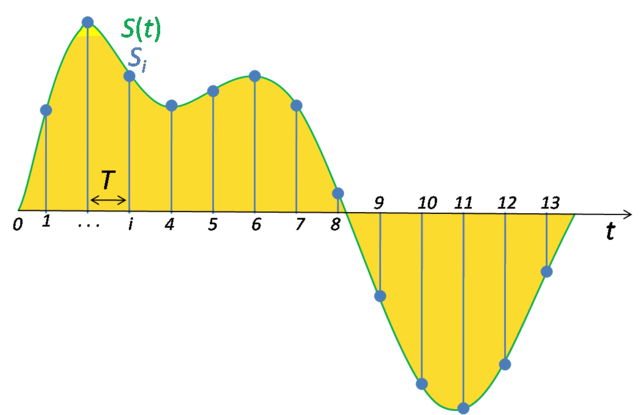
\includegraphics[width=0.6\textwidth]{Signal_Sampling}
%   \caption{Δειγματοληψία ενός αναλογικού σήματος}
%   \label{fig:sampling}
% \end{figure}

% \begin{theorem}[Shannon-Nyquist]
% 	\label{thrm:shannon-nyquist}
% 	Ένα σήμα με μέγιστη συχνότητα $f_{max}$ μπορεί να ανακτηθεί από τα δείγματά του, αν αυτά ληφθούν με συχνότητα $f_s>2f_{max}$, ή αλλιώς με περίοδο $T_s<\frac{1}{2f_{max}}$. \cite{proakis_sampling}
% \end{theorem}